\documentclass[conference]{IEEEtran}
\IEEEoverridecommandlockouts
% The preceding line is only needed to identify funding in the first footnote. If that is unneeded, please comment it out.
\usepackage{cite}
\usepackage{amsmath,amssymb,amsfonts}
\usepackage{algorithmic}
\usepackage{graphicx}
\usepackage{textcomp}
\usepackage{xcolor}
\usepackage{float}
\usepackage{caption}
\usepackage{amsmath}
\usepackage{dirtytalk}
\usepackage{tikz}
\def\BibTeX{{\rm B\kern-.05em{\sc i\kern-.025em b}\kern-.08em
    T\kern-.1667em\lower.7ex\hbox{E}\kern-.125emX}}
\begin{document}

\newcommand{\RN}[1]{%
  \textup{\uppercase\expandafter{\romannumeral#1}}%
}

\title{CENG 435 - Data Communications and Networking\\
Term Project - Part \RN{2}}

\author{
\IEEEauthorblockN{Sina Sehlaver}
\IEEEauthorblockA{\textit{Department of Computer Engineering}\\
\textit{Middle East Technical University}\\
2099729}
\and
\IEEEauthorblockN{Beyazit Yalcinkaya}
\IEEEauthorblockA{\textit{Department of Computer Engineering}\\
\textit{Middle East Technical University}\\
2172138}
}

\maketitle

\begin{abstract}
    In this project, we present our own reliable data transfer protocol design that is built on top of UDP. A modified version of selective repeat is implemented, pipelining method is used, multi-homing is practiced, single-ACKs are used, and an auto-link-down detection is developed. The performance of this reliable data transfer protocol of our own is measured with two experiments. The first experiment examined the performance through one link, whereas the second experiment showed the effects of using multi-homing with two links. As a result, we concluded that in both experiments the increase in packet loss increases the file transfer time considerably and creates an overhead for the performance. Furthermore, the comparison between the two experiments point out the benefits of using multi-homing in order to increase the utilisation of links and shorten file transfer time.

\end{abstract}

\section{Introduction}


    This paper explains the details of the second part of the term project. In this part of the term project, we are expected to send a file with exactly five Mb file size from source to destination with a self-designed reliable data transfer protocol on top of UDP, in a given network topology. Our motivation was to get familiar with the reliable data transfer process and its challenges. In accordance with our motivation, we have designed our own reliable data transfer protocol that includes our combination of modified methods such as selective repeat, pipelining and multi-homing. On top of these, we have created our own methods such as auto-link-down detection. Since the experiment is extremely case-specific as in we will always send exactly five Mbs (5000000 bytes), we have implemented our reliable data protocol in accordance with these specifications. Our protocol, transfers the file in a reliable fashion, as promised.
    
    Multi-homing is one of the important aspects of our reliable data protocol. Multi-homing is implemented in a fashion that it splits the file into two parts and sends them separately. We have implemented the protocol in a way that in the case of one of the routers being down (at most one can be down), it will redirect the file transmission traffic onto the other \say{alive} router so that the reliable data transfer is not interrupted. In order to examine the performance of our protocol from multiple view-points, we have conducted two experiments. The first one is conducted in a way that it transfers the file through one router, that is $r3$. The latter one, on the other hand, transfers the file through two distinct routers, namely $r1,r2$. Both of them measure the performance of our reliable transfer protocol, however the second one also measures the multi-homing method's performance.
    
    For both of the experiments, we have used the \say{tc/netem} setup configuration in order to emulate packet loss with delays on the links. We have specified the packet loss percentages and delay durations when calling \say{tc/netem}. With the help of the emulation, we were able to observe the relationship between packet loss percentage and file transfer time. Since our packet based protocol is practicing reliable data transfer, each packet must arrive to the destination and thus, packet loss directly affects the file transfer time.
    
    When we compare the two experiments, we see that multi-homing has a positive impact on the performance of our protocol since it reduces the file transfer time, as expected. We have repeated our experiments such that the error margin of our results did not exceed $0.1$ with a confidence interval of 95\% and gathered the data with this statistical assurance.
    
    The outline of our paper is as follows; in the second section we will explain the methodologies we have used in these experiments, in the third section we give specific implementation details and justify them, in the fourth section we report and discuss our experimental results and section 5 concludes the paper.
    


\section{Methodology}


\begin{figure*}[t]
\caption*{Code Segment for Multi-homing, Pipelining and Automatic Link Down Detection}
\centerline{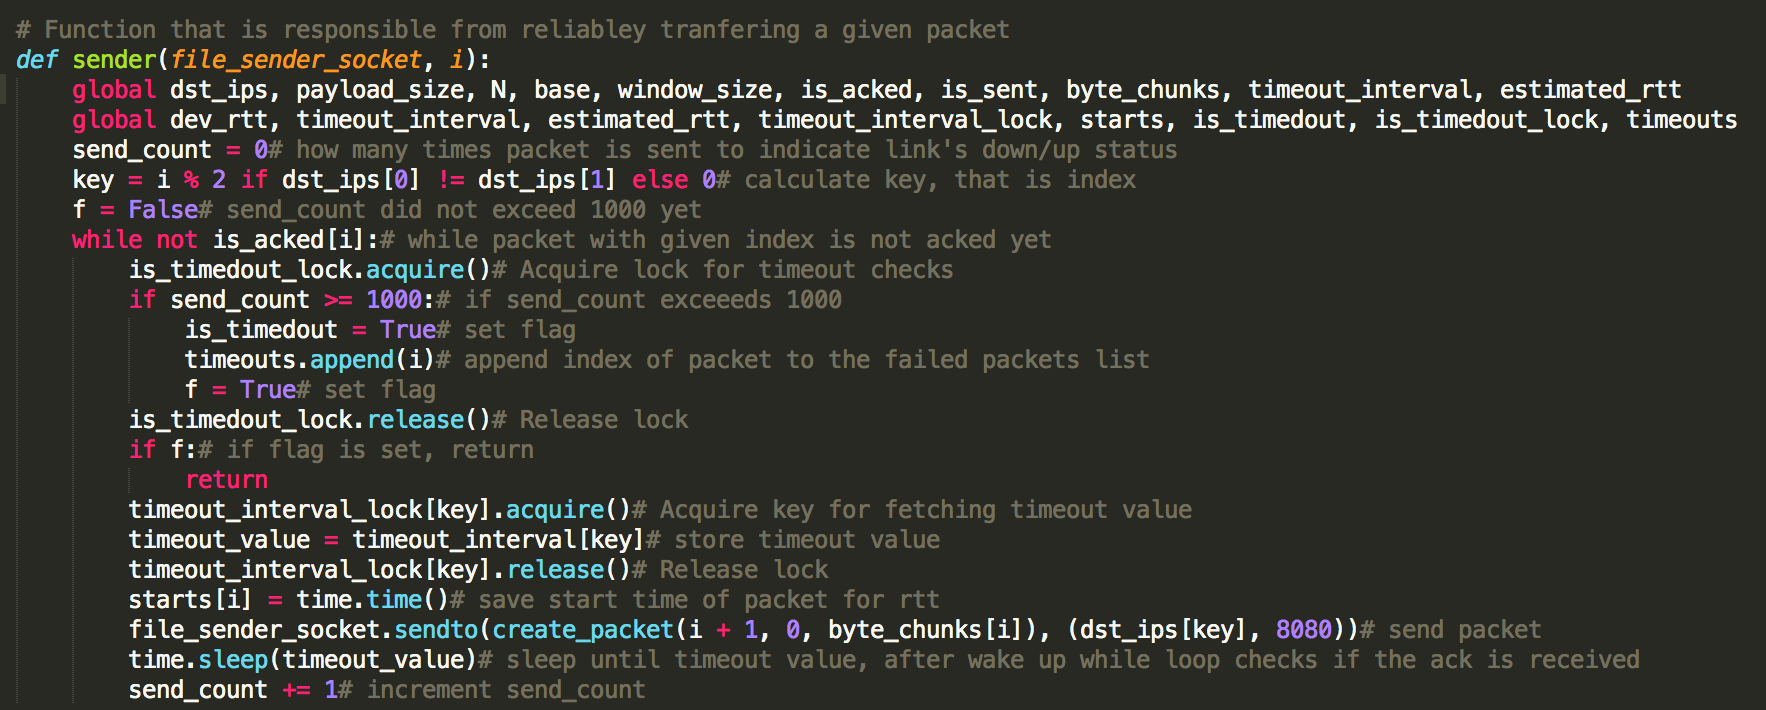
\includegraphics[width=\textwidth]{sender.png}}
\label{graph}
\end{figure*}

    This section describes the design and logic of the methods used in the experiments. We have reserved resources through the GENI platform with the topology described inside the XML format topology file. We have used the specific IP addresses configured by this file to connect each node in our topology to each other. 

    In accordance with the specifications given to us, that is sending a file from $s$ node to $d$ node with exactly five Mbs file size in the given network topology, we have designed a protocol which will ensure reliable data transfer. We have implemented pipelining, multi-homing and auto-link-down detection. We have setup two experiments to test our reliable data transfer protocol. The first one aimed to measure the performance of the protocol with respect to the packet loss through one path whereas the second one used two distinct paths while sending the data in order to measure the effects of multi-homing on the performance. 
    
    In these experiments, in order to configure specific packet loss percentages that are given to us, we have used \say{tc/netem} command. This command enabled us to emulate packet loss (with a specified rate), during the transmission of packets between the nodes in the network. Our reliable data transfer protocol repeatedly sent the lost packets in order to compensate the emulated loss. Through experimentation, we have observed that this repeated transmission, and therefore, the packet loss had a negative effect on the file transfer time. 
    
    For pipelining, with an inspiration from selective repeat, we have created our own method. Just as it is with selective repeat; our sender, sends the packets that are within a window with a pre-determined size in a pipelined fashion, that is, it sends two consecutive packets without waiting for the arrival of their corresponding ACK messages. Each packet inside this window has a timeout duration that is calculated dynamically in accordance with the network's state and during this timeout period, the sender waits for their ACK messages to arrive. In case of an ACK message not arriving during the timeout duration, it will resend the packet. For the packets that received their ACK messages, we have increased the \say{base} such that none of the packets that are not ACKed would be left outside of the window. 
    
    For the multi-homing method, we have split the file into two, in an abstract fashion. The packets that have odd indexes used one distinct path while the even indexed packets used the other path. This division of file to paths, actually enabled a faster transmission of the file to the destination without exhausting the paths. For the case of \say{at most one of the links being down} in this multi-homing part, we have come up with a method that prevents the interruption of the file transfer. Our method is as follows; if a packet does not receive its ACK message during its timeout period, a 1000 consecutive times, we deduce that that link is \say{down} and we redirect the file transmission to the other link that we believe is up.
    
    We did not use any \say{NAK} messages in our implementation but only \say{ACK} messages. For the buffering, we used global arrays inside the python script of node $d$ that holds the received byte chunks. The case of failure in receiving a packetm is handled with timeouts. The timeout value is calculated dynamically after each packet transmission by using following equations.
    
    \begin{equation}
        \begin{split}
            EstimatedRTT & = (1-\alpha ) EstimatedRTT\\
            & \qquad \qquad + \alpha SampleRTT\\
            DevRTT & = (1-\beta ) DevRTT \\ &  + \beta | SampleRTT - EstimatedRTT |\\
            TimeoutInterval & = EstimatedRTT + 4DevRTT
        \end{split}
    \end{equation}
    
    
    where we used $\alpha = 0.125$ and $\beta = 0.25$.
  
    For the calculation of round-trip time (RTT); for each packet we save the time just before we send it and when the corresponding ACK message of the packet is received, we calculate the time between these two events and that becomes our $SampleRTT$. After the calculation of $SampleRTT$ we apply the equations above to get the $TimeoutInterval$. For the distinct paths in our second experiments, we did the calculations for each of them separately.
    
    

\begin{figure*}[t]
\caption*{Margin of Error Tables}
\centerline{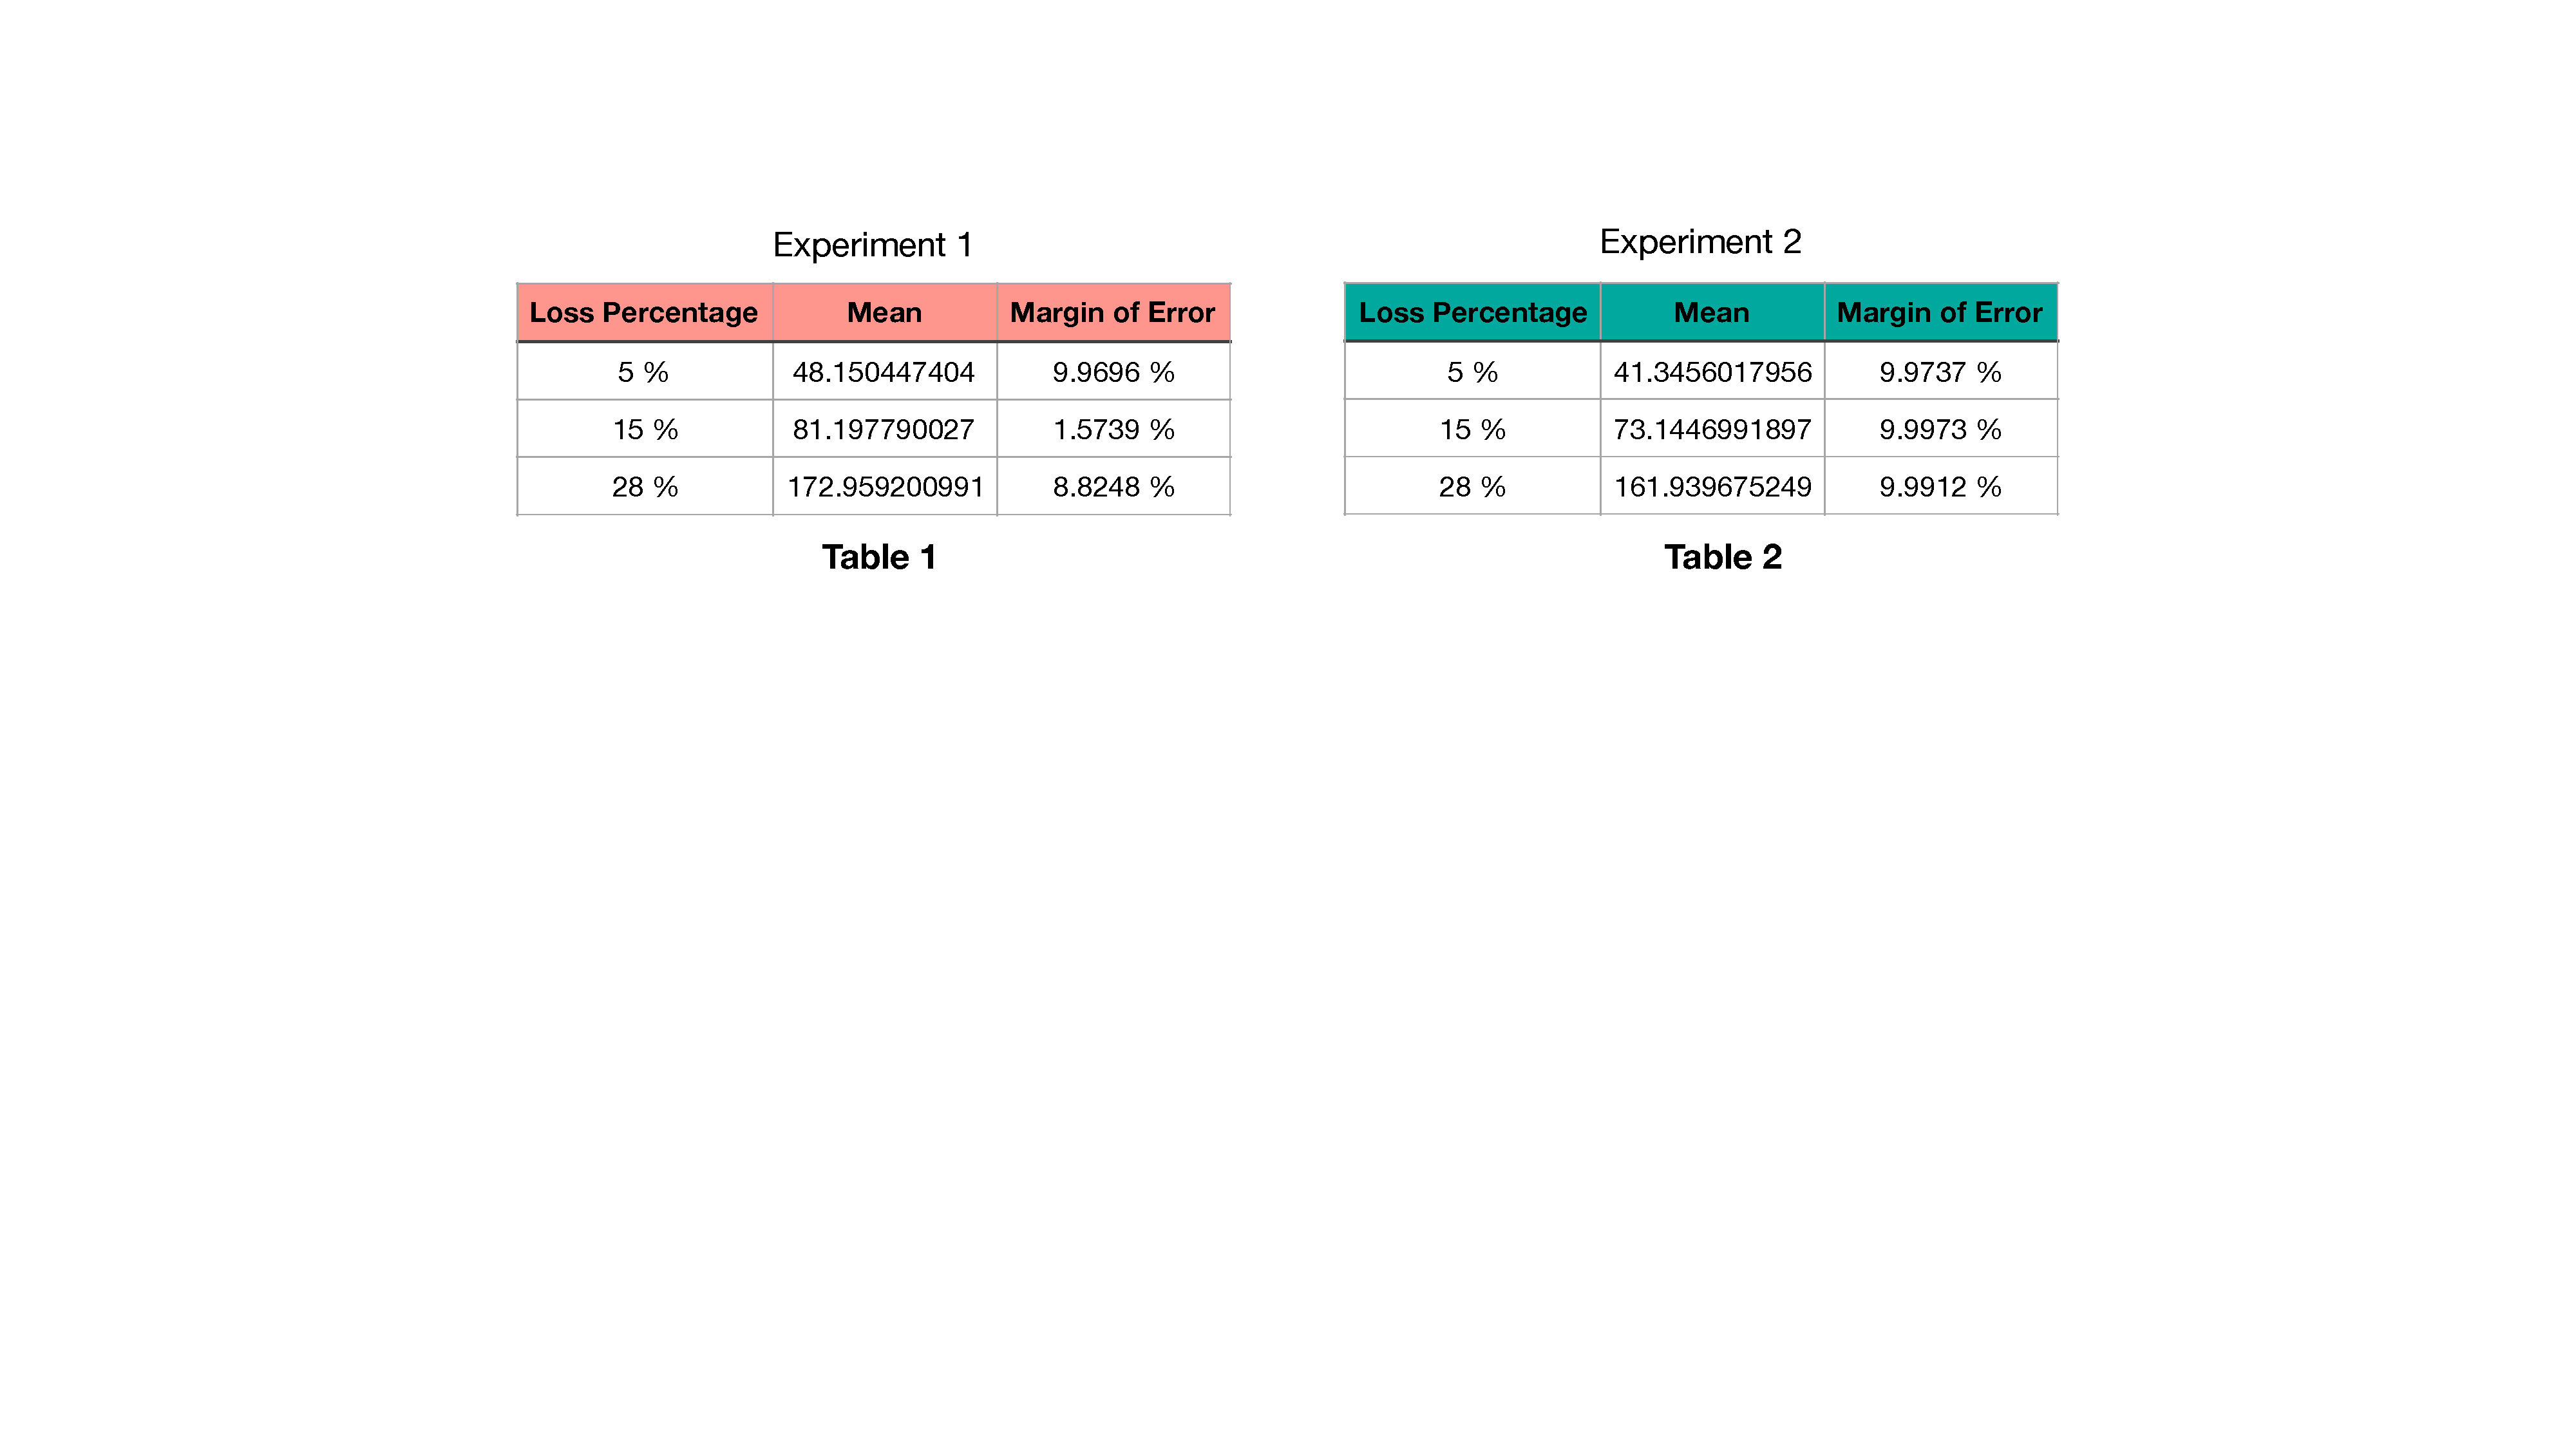
\includegraphics[width=\textwidth]{tables.pdf}}
\label{graph}
\end{figure*}
    
    The packets consist of a header and a payload. 
    
    Header consists of; 
    \begin{itemize}
        \item Sequence number (2 bytes)
        \item ACK number (2 bytes)
        \item Length (2 bytes)
        \item Checksum (32 bytes)
    \end{itemize} 
    
    Payload consists of 512 bytes of data chunk.
    
    For the checksum, we have used the \say{md5} sum method. It checks whether the payload (and only the payload) is received without any corruption. It is a well-known and reliable method that is widely-used. 
    
    When all packets receive their corresponding ACK messages, sender sends a packet with sequence and ACK number both $0$ in a reliable fashion (resends it until the arrival of a corresponding ACK message) in order to inform the receiver that the transmission is done. When receiver receives this message, as opposed to the sender, unreliably sends a packet with the same configuration (seq and ACK no $0$) and terminates. If the sender receives this new packet sent from the receiver, it terminates safely. However, in the case of not receiving this new packet, the sender continues to try to send the same packet over and over until it sends it $1000$ consecutive times that result in timeout.
    
    After that the file transmission is done with the above mentioned methods and conventions, sender reports the file transfer time. This file transfer experiment is conducted repeatedly until the results ensure a margin of error less than $0.1$ with a confidence interval of 95\%. The number of repetition is also calculated dynamically, that is, we calculate the margin of error after each new experiment result and stop the execution when the conditions are satisfied. The reported numbers are discussed in the experiment results section.
    
\section{Implementation}

    
        This section of the report, explains the implementation details of the methodology section. We used Python3 and Bash scripts, each Python3 script \say{main.py} is run with a Bash script \say{start.sh} for each corresponding node.
    
        Several modules were used:
            \begin{itemize}
                \item socket module for the transmission
                \item threading module for concurrency
                \item struct module for packet header construction
                \item sys module for input arguments
                \item time module for round trip time, file transfer time and timeout
                \item hashlib module for md5 calculation
                \item statistics for statistical tools
                \item math for mathematical tools 
                \item tc/netem command to emulate network packet loss and delay
            \end{itemize}
        
        We have created a \say{README.md} file, explaining the structure of the scripts and the instructions for the reproduction of the experiment environment. Each script also include comments that elaborate on the functionality.
      
      

\begin{figure*}[t]
\caption*{File Transfer Time vs Packet Loss Percentage Experiments}
\centerline{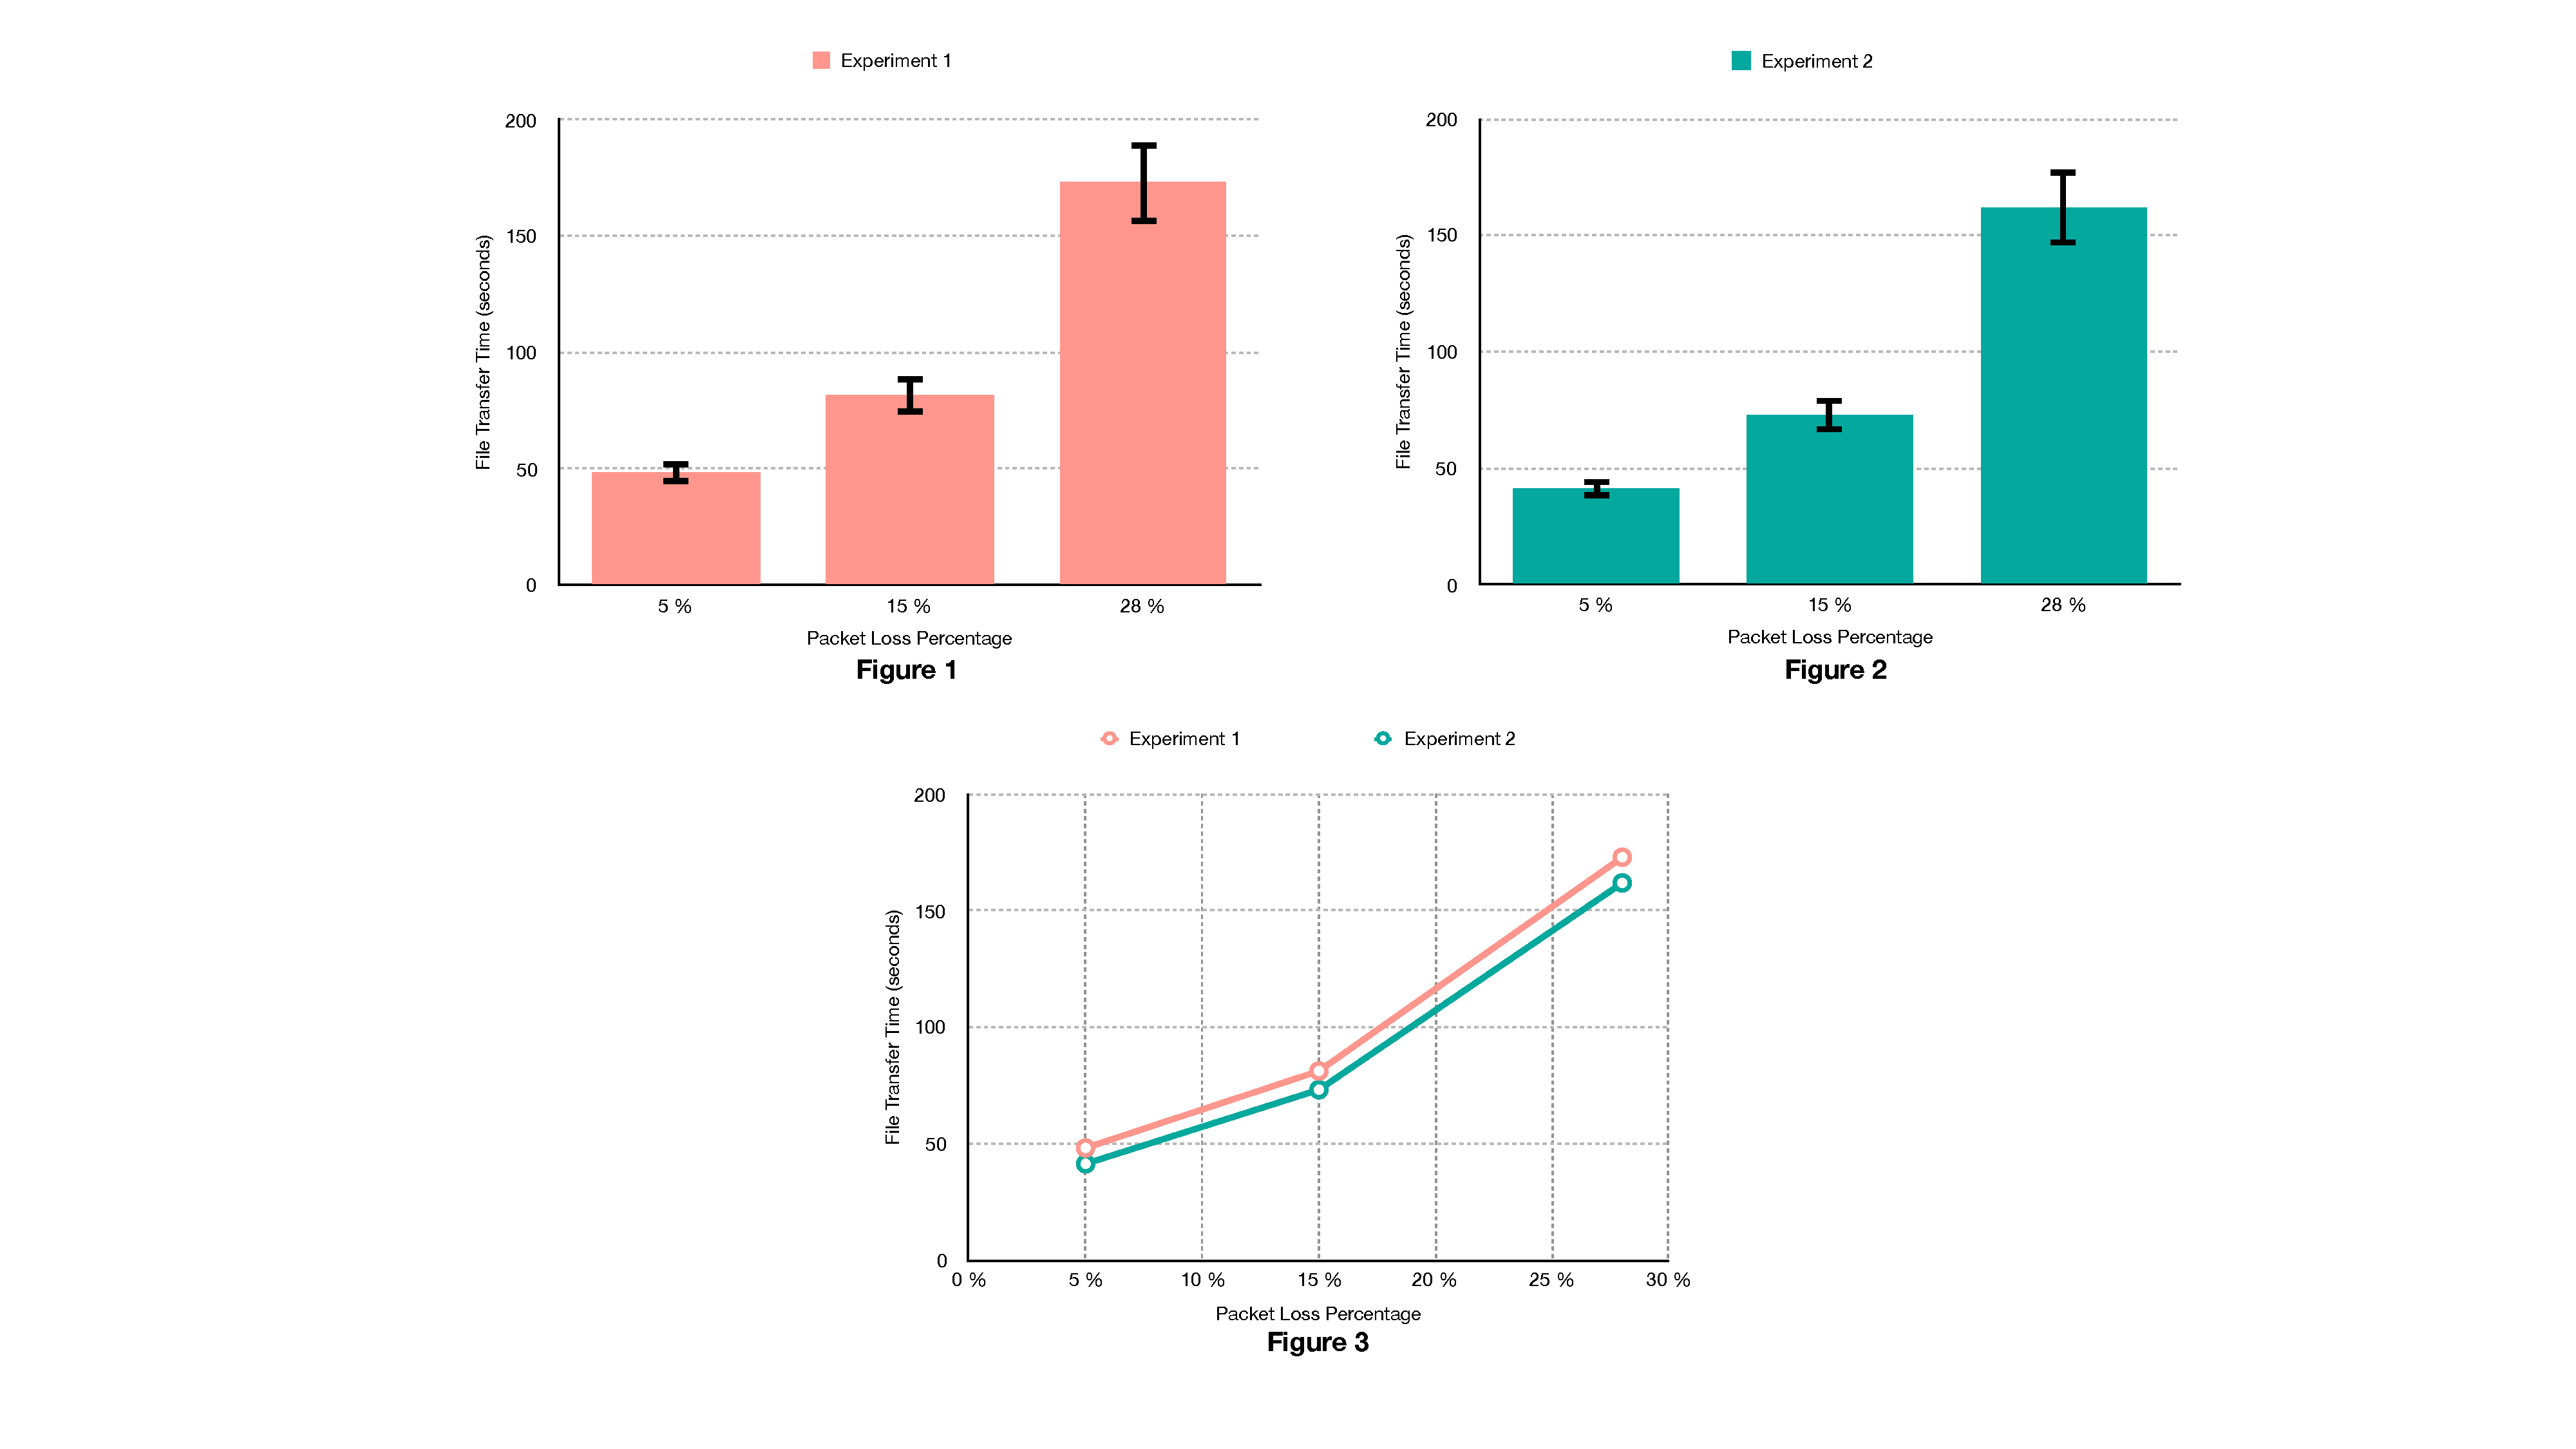
\includegraphics[width=\textwidth]{exps.pdf}}
\label{graph}
\end{figure*}
        
    $r1,r2,r3$ nodes run a simple python script that includes a routing table for the correct redirection of the packets and uses this routing table to send the arriving packets to their destinations. This python script is called from the bash script \say{start.sh}. This bash script calls other bash scripts that configure the network settings of each connection of that node, respectively and in order: reset, initialisation and configuration. The script \say{start.sh} takes loss percentage as argument.\\
    These setting scripts use \say{tc/netem} commands: 
    
    \begin{itemize}
        \item first reset all the previous settings with \say{del} command
        \item second initialise with \say{add} command
        \item finally configure loss percentages and delays with \say{change} command
    \end{itemize}
    
    Node $s$ also has the same reset, init and config scripts that $r1,r2,r3$ have. Alongside with those, it has a \say{main.py} that is different from all others and a \say{start.sh} which also has a different implementation from all others. \\
    The script \say{start.sh} accepts the following arguments as its input arguments: 
        \begin{itemize}
            \item Experiment type
            \item Loss percentage
            \item Input file name
            \item Margin of error threshold
        \end{itemize}
    
    
    After calling the setting bash scripts mentioned above, the \say{start.sh} script calls \say{main.py} with input arguments; experiment type, input file name and margin of error threshold. \say{main.py} checks whether margin of error threshold is $-1$, if so, it deduces that the experiment is supposed to run only once. On the other hand if it is a non-negative value, the experiment is repeated until the margin of error falls under that threshold.
    
    The script \say{main.py} in $s$ splits the file into byte chunks and then creates an \say{ACK receiver thread}. When an ACK message is received, this thread marks the packet's ACK message as \say{received} inside a global array that holds the states of ACK messages of all packets. At the same time, when an ACK message is received, this receiver thread calculates the corresponding packet's round trip time and then does the calculations mentioned in the methodology section to fetch the timeout value. After these, \say{file sender} function is called. This function, creates a special \say{sender} thread in order to send each byte chunk with the modified selective repeat method that we have mentioned above. The sender thread takes a specific byte chunk, creates a packet such that this byte chunk is its payload and then reliably sends it to the destination.\\ In order to reliably send the file, while the packet's ACK message is not received; 
    \begin{itemize}
        \item It sends the packet
        \item sleeps for the $timeout$ duration
    \end{itemize}
    
    If the ACK message is not received by the end of the sleep, it re-sends the packet. This re-transmission is counted as $timeout$ and if a packet is re-sent $1000$ times because of $timeout$, the file sender function is informed via a global variable (\textit{Code segment figure}) so that the file sender function can detect it in its main loop and redirect its remaining file transfer to the link that is up. When all ACK messages arrive to $s$, $s$ sends a packet with sequence and ACK number $0$ to $d$ so that $d$ is informed that the file transmission is over.
    
    Node $d$ also has the same reset, init and config scripts that $r1,r2,r3$ have. Alongside with those, it has a \say{main.py} that is different from all others and a \say{start.sh} which also has a different implementation from all others. \\
    The script \say{start.sh} accepts the following arguments as its input arguments: 
        \begin{itemize}
            \item Loss percentage
            \item Output file name
            \item Repetition count
        \end{itemize}
    
    After calling the setting bash scripts mentioned above, the \say{start.sh} script calls \say{main.py} with input arguments; output file name and repetition count. \say{main.py} checks whether repetition count is $-1$, if so, it runs in an infinite loop. On the other hand if it is a non-negative value, the experiment is repeated as many times as the value. \say{main.py} calls the file receiver function. This function checks the checksums of received packets. If they are intact and the file receiver function did not receive another packet with the same sequence number before, it puts that packet at the corresponding index in a fixed-size global byte chunk array. If the checksum indicates that the file is corrupted, the packet is ignored. In any other scenario, that is file is received without corruption, file receiver function sends an ACK message through the corresponding path to the corresponding node for each and every packet it receives. When a packet that has a sequence and ACK number of $0$ arrives to the file receiver, it deduces that the file transmission is over; it creates a file with the specified output file name, writes the data in the byte chunks to that file and terminates. In accordance with the case-specific implementation and the modified selective repeat method, the byte chunk array inside $d$ resembles a bookshelf; in order to have the entire file, it is sufficient to put every book (payload) that arrives, into its corresponding place (index). 
    
    In our implementation, after that the file transfer is done, each script terminates and the script inside $s$ prints the file transfer time to the \say{stdout}. If one wants to execute this flow for just one file transfer; one should set margin of error threshold to $-1$ in $s$ and repetition count to $1$ in $d$. This way, one file transfer is completed reliably and all the scripts in the nodes terminate. Routing tables before and after link down operation in computers r1 and r2 are given in the Appendix with their related commands.


\section{Experiment Results}

     In this section we present our experiment results of experiment one and two in two subsections. We give corresponding graphs and tables and discuss the results. Figures \textit{1} and \textit{2} show the margin of error as $10\%$ for each packet loss percentage since our experiments fall inside that region. However, as explained in the methodology part, we have stopped our experiments only after the margin of error dropped below our threshold $0.1$. Thus, although the figures \textit{1} and \textit{2} show $10\%$ for each, the real margins of error are reported in \textit{Table 1} and \textit{Table 2} in detail.

\subsection{Experiment I}
    
    In this experiment we have transfered the file through $s-r3-d$. We have emulated packet loss percentages of $5\%, 15\%$ and $28\%$. These emulations were done using the \say{tc/netem} command as explained in the methodology section. 

    The observation from the graph shows us that; as packet loss percentage increases, the file transfer time also increases. It is an expected behaviour from a reliable data transfer protocol since it will try to send the lost packets until it ensures the arrival of the packets. However this behaviour is observed to increase the overhead as the loss percentage grows.
    
    
\subsection{Experiment II}

    In this experiment, as opposed to the first one, we send the file through two distinct paths, namely; $s-r1-d$ and $s-r2-d$. The experiments were conducted after the respective configurations were done on the network. Both of the mentioned distinct paths were up during the experiment. 
    
    The graph in \textit{Fig. 2} shows a similar behaviour to the one in \textit{Experiment I} and shows us the same direct relationship between packet loss percentage and file transfer time as expected. 
    
\subsection{Comparison}
    From the graph that compares the two experiments in \textit{Fig. 3}, we can clearly infer that \textit{Experiment II} is faster than \textit{Experiment I}. The reason behind this is that the file division of multi-homing that uses 2 links to transfer separate parts of the file, utilises more links than that of \textit{Experiment I} and thus it is faster. We can also observe that the difference between the two experiments in time is almost the same for every packet loss percentage, revealing the independency of multi-homing and packet loss. 
  

\section{Conclusion}
    
    This paper presents our own reliable data transfer protocol that we built on top of UDP. We used a modified version of selective repeat, we sent our files with pipelining method, we utilised more links by practicing multi-homing, we used single-ACKs and we implemented an auto-link-down detection of our own for reliability. We have tested the performance of our reliable data transfer protocol with two experiments. While the first experiment measured the performance of our reliable data transfer protocol through one link, the second experiment pointed out the effects of using multi-homing with two links. When we elaborate on the results of the experiments, as a common aspect, we see that in both experiments the increase in packet loss drastically increases the file transfer time, creating an overhead that negatively affects the performance. In addition to that, the difference between the two experiments reveal the fact that putting multi-homing to use increases our utilisation of network links and the overall performance by decreasing the file transfer time.




    
    
\begin{figure*}[t]
\caption*{\textbf{APPENDIX}}
\centerline{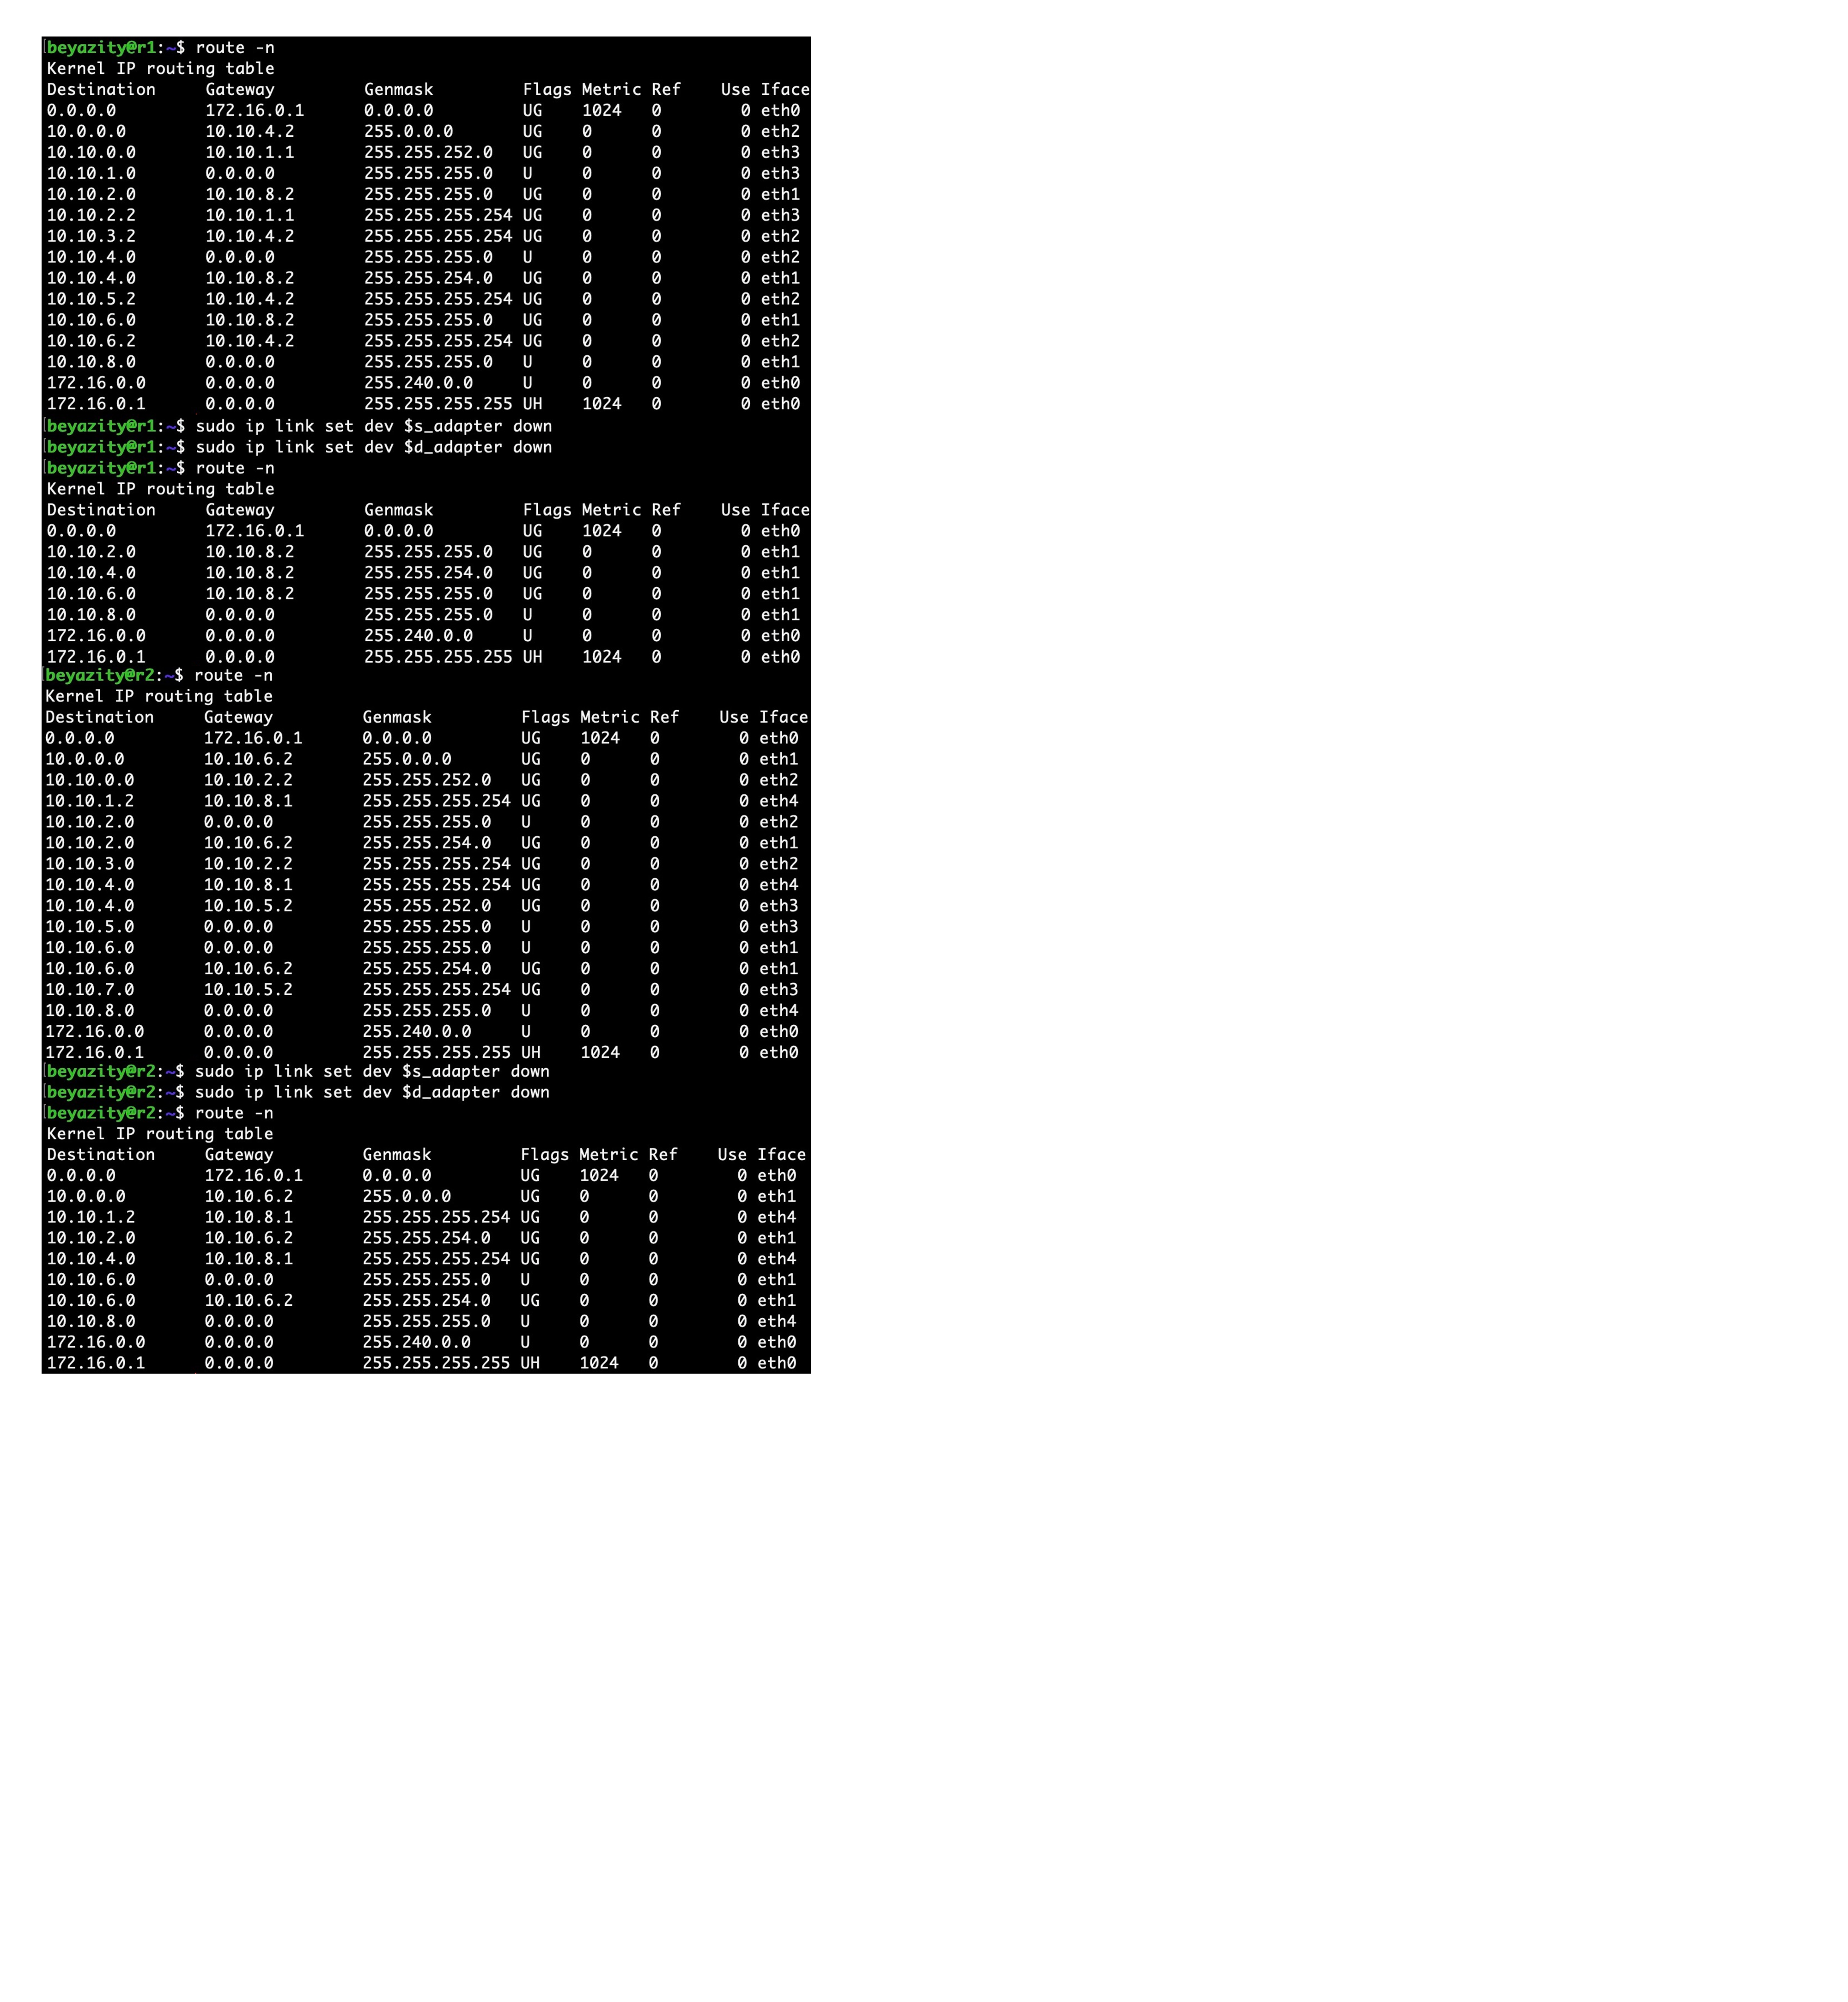
\includegraphics[width=360pt]{screenshots.pdf}}
\label{graph}
\end{figure*}



\end{document}
